\documentclass[a4 paper]{article}

% Set target color model to RGB
\usepackage[inner=2.0cm,outer=2.0cm,top=2.5cm,bottom=2.5cm]{geometry}
\usepackage{setspace}
\usepackage[rgb]{xcolor}
\usepackage{verbatim}
\usepackage{subcaption}
\usepackage{amsgen,amsmath,amstext,amsbsy,amsopn,tikz,amssymb,tkz-linknodes}
\usepackage{fancyhdr}
\usepackage[colorlinks=true, urlcolor=blue,  linkcolor=blue, citecolor=blue]{hyperref}
\usepackage[colorinlistoftodos]{todonotes}
\usepackage{rotating}
%\usetikzlibrary{through,backgrounds}
\hypersetup{%
pdfauthor={Nabeel Warsalee},%
pdftitle={COMP3005 Final Project Report},%
pdfkeywords={Tikz,latex,bootstrap,uncertaintes},%
pdfcreator={PDFLaTeX},%
pdfproducer={PDFLaTeX},%
}
%\usetikzlibrary{shadows}
% \usepackage[francais]{babel}
\usepackage{booktabs}
\newcommand{\ra}[1]{\renewcommand{\arraystretch}{#1}}

\newtheorem{thm}{Theorem}[section]
\newtheorem{prop}[thm]{Proposition}
\newtheorem{lem}[thm]{Lemma}
\newtheorem{cor}[thm]{Corollary}
\newtheorem{defn}[thm]{Definition}
\newtheorem{rem}[thm]{Remark}
\numberwithin{equation}{section}

\newcommand{\homework}[6]{
   \pagestyle{myheadings}
   \thispagestyle{plain}
   \newpage
   \setcounter{page}{1}
   \noindent
   \begin{center}
   \framebox{
      \vbox{\vspace{2mm}
    \hbox to 6.28in { {\bf COMP 3005:~Database Management Systems \hfill {\small (#2)}} }
       \vspace{6mm}
       \hbox to 6.28in { {\Large \hfill #1  \hfill} }
       \vspace{6mm}
       \hbox to 6.28in { {\it Instructor: {\rm #3} \hfill Name: {\rm #5}, ID: {\rm #6}} }
       %\hbox to 6.28in { {\it TA: #4  \hfill #6}}
      \vspace{2mm}}
   }
   \end{center}
   \markboth{#5 -- #1}{#5 -- #1}
   \vspace*{4mm}
}

\newcommand{\problem}[2]{~\\\fbox{\textbf{Q #1}}\hfill (#2 points)\newline\newline}
\newcommand{\subproblem}[1]{~\newline\textbf{(#1)}}
\newcommand{\D}{\mathcal{D}}
\newcommand{\Hy}{\mathcal{H}}
\newcommand{\VS}{\textrm{VS}}
\newcommand{\solution}{~\newline\textbf{\textit{(Solution)}} }

\newcommand{\bbF}{\mathbb{F}}
\newcommand{\bbX}{\mathbb{X}}
\newcommand{\bI}{\mathbf{I}}
\newcommand{\bX}{\mathbf{X}}
\newcommand{\bY}{\mathbf{Y}}
\newcommand{\bepsilon}{\boldsymbol{\epsilon}}
\newcommand{\balpha}{\boldsymbol{\alpha}}
\newcommand{\bbeta}{\boldsymbol{\beta}}
\newcommand{\0}{\mathbf{0}}


\begin{document}
\homework{COMP3005 Final Project Report}{Due: Dec. 10th, 2021 (11:59 PM)}{Ahmed El-Roby}{}{}{}

\section*{Introduction}
This is the project report for the COMP3005A Final Project for the Fall 2021 term.\\
The group for this project consists of the following members...\\

\noindent\underline{\textbf{Group Members}}
\begin{itemize}
	\item Aaron Buitenwerf (101106637)
	\item Hadi Cheaito (101110188)
	\item Nabeel Warsalee (101103167)
\end{itemize}

\noindent All project files and source code can be found at the following \href{https://github.com/COMP3005A-Project/bookstore}{Github repository}...

\section{Conceptual Design}
For the design of this database, we took a straightforward approach and attempted to keep it as simple as we could. We created four main entities that compose the bulk of what the program requires. There are then relationships and minor entities that help provide more information for our main entities while also avoiding redundancy.\\

\noindent The book entity contains all the information regarding the books in our system. The primary key for this entity is the isbn number. The book entity forms relationships with the publisher entity, via the relationship of a book being published by a given publisher and is also connected to the order relation via the relationship books\_in\_order.\\

\noindent The publisher entity contains all the information regarding the publishers in our system. The primary key for this entity is the name of the publisher. The publisher entity forms relationships with the book entity as mentioned earlier and is also connected to the bank\_account relation via the relationship account\_of.\\

\noindent The order entity contains all the information regarding the book orders in our system. The primary key for this entity is the order id. The order entity forms relationships with the book entity as mentioned earlier via the books\_in\_order relationship and is also connected to the customer relation via the relationship order\_of.//

\noindent Finally there is the customer entity which contains all the information regarding the customers in our system. The primary key for this entity is the email of the user. The customer entity forms relationships with the order entity as mentioned earlier via the order\_of relationship.\\

\noindent\underline{\textbf{Assumptions Made}}\\
In this section we list all the assumptions that were made for certain aspects of the problem statement. These assumptions reflect how we designed and organized our database for this project.

\begin{itemize}
	\item A book can only have one publisher
	\item All books with same title have the same ISBN
	\item Assume an order can only have one of the same book (i.e., user cannot buy two copies of the same book in one order)
	\item Each publisher has only one bank account
	\item There is only one set of reports made per publisher
	\item Tracking information for an order is just its shipping id
\end{itemize}

\noindent\underline{\textbf{ER Diagram}}\\
The following is the Entity-Relationship Diagram created to model the entities and relationships from the provided problem statement using the assumptions we have outlined above.\\

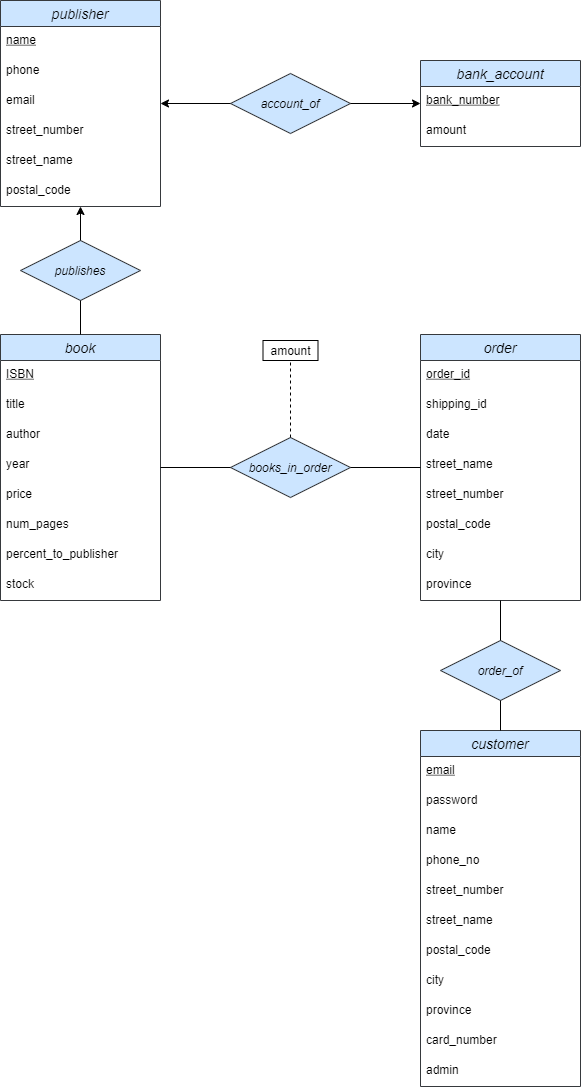
\includegraphics[scale=0.5]{../Diagrams/ER-diagram-bookstore-comp3005-finalproject.drawio.png}\\

\section{Reduction to Relation Schemas}
Here are the relation schemas gained from reducing our ER diagram into relations... (Note: Primary keys are underlined)\\

book(\underline{isbn}, title, author, genre, year, price, num\_pages, publisher\_name, stock, percent\_to\_publisher)\\
\indent order(\underline{order\_id}, email, shipping\_id, date, street\_number, street\_name, postal\_code, city, province)\\
\indent books\_in\_order(\underline{order\_id}, \underline{isbn}, amount)\\
\indent customer(\underline{email}, password, name, phone, street\_number, street\_name, postal\_code, city, province, card\_number, admin)\\
\indent publisher(\underline{name}, phone, bank\_number, email, street\_number, street\_name, postal\_code)\\
\indent bank\_account(\underline{bank\_number}, amount, debt\_amount)\\

\section{Normalization of Relation Schemas}

\underline{\textbf{Functional Dependencies}}\\

\noindent\emph{book}

isbn $\rightarrow$ title, author, genre, year, price, num\_pages, publisher\_name, stock, percent\_to\_publisher\\
\indent title, author $\rightarrow$ isbn, genre, year, price, num\_pages, publisher\_name, stock, percent\_to\_publisher\\

\noindent\emph{order}

order\_id $\rightarrow$ email, shipping\_id, date, street\_number, street\_name, postal\_code, city, province\\
\indent shipping\_id $\rightarrow$ email, order\_id, date, street\_number, street\_name, postal\_code, city, province\\
\indent postal\_code $\rightarrow$ city, province\\

\noindent\emph{books\_in\_order}

order\_id, isbn $\rightarrow$ amount\\

\noindent\emph{customer}

email, password $\rightarrow$ name, phone, street\_number, street\_name, postal\_code, city, province, card\_number, admin\\
\indent postal\_code $\rightarrow$ city, province\\

\noindent\emph{publisher}

name $\rightarrow$ email, phone, bank\_number, street\_number, street\_name, postal\_code\\
\indent email $\rightarrow$ name, phone, bank\_number, street\_number, street\_name, postal\_code\\

\noindent\emph{bank\_account}

bank\_number $\rightarrow$ amount, debt\_amount\\

\noindent\underline{\textbf{Good Normal Form Check and Decomposition}}\\

\noindent\underline{\emph{book}}\\

\noindent 1st FD...\\
\indent Closure of \emph{isbn}, (\emph{isbn})+ = (isbn, title, author, genre, year, price, num\_pages, publisher\_name, stock, percent\_to\_publisher)\\
\indent Since the closure of isbn includes all attributes in the relation, it means isbn is a superkey for the relation and it complies with BCNF.\\

\noindent 2nd FD...\\
\indent Closure of \emph{title, author}, (\emph{title, author})+ = (isbn, title, author, genre, year, price, num\_pages, publisher\_name, stock, percent\_to\_publisher)\\
\indent Since the closure of (title, author) includes all attributes in the relation, it means (title, author) is a superkey for the relation and it complies with BCNF.\\

\noindent Since all FD's for this relation satisfy the conditions for BCNF, this table is already in BCNF. Since the table is already in BCNF and no decomposition was done, all dependencies are preserved.\\

\noindent\underline{\emph{order}}\\

\noindent 1st FD...\\
\indent Closure of \emph{order\_id}, (\emph{order\_id})+ = (order\_id, email, shipping\_id, date, street\_number, street\_name, postal\_code, city, province)\\
\indent Since the closure of order\_id includes all attributes in the relation, it means order\_id is a superkey for the relation and it complies with BCNF.\\

\noindent 2nd FD...\\
\indent Closure of \emph{shipping\_id}, (\emph{shipping\_id})+ = (order\_id, email, shipping\_id, date, street\_number, street\_name, postal\_code, city, province)\\
\indent Since the closure of shipping\_id includes all attributes in the relation, it means shipping\_id is a superkey for the relation and it complies with BCNF.\\

\noindent 3rd FD...\\
\indent Closure of \emph{postal\_code}, (\emph{postal\_code})+ = (postal\_code, city, province)\\
\indent Since the closure of postal\_code does not include all attributes in the original relation, it means postal\_code is not a superkey for the relation and thus violates the conditions for BCNF. We will need to decompose this relation.\\

\noindent\underline{Decomposition}\\
Decompose into two new relations, order and region\_order...

order(order\_id, email, shipping id, date, street\_number, street\_name)\\
\indent region\_order(postal\_code, city, province)\\

\noindent Now none of the functional dependencies violates BCNF since postal\_code is now a superkey for the relation called \emph{region\_order}.\\

\noindent\underline{Dependency preservation}\\

\begin{enumerate}
	\item Check FD: order\_id $\rightarrow$ email, shipping\_id, date, street\_number, street\_name, postal\_code, city, province\\
	Start with result $r =$ order\_id\\
	
	$R_{1} = $(order\_id, email, shipping\_id, date, street\_number, street\_name, postal\_code)\\
	$t = (result \cap R_{1})+ \cap R_{1}$\\
	$t =$ (order\_id, email, shipping\_id, date, street\_number, street\_name, postal\_code)\\
	result $=$ (order\_id) $\cup$ (order\_id, email, shipping\_id, date, street\_number, street\_name, postal\_code)\\
	result $=$ (order\_id, email, shipping\_id, date, street\_number, street\_name, postal\_code)\\
	
	$R_{2} =$ (postal\_code, city, province)\\
	$t = (result \cap R_{2})+ \cap R_{2}$\\
	$t =$ (postal\_code, province, city)\\
	result $=$ (order\_id, email, shipping\_id, date, street\_number, street\_name, postal\_code) $\cup$ (postal\_code, province, city)\\
	result $=$ (order\_id, email, shipping\_id, date, street\_number, street\_name, postal\_code)\\
	
	Since result contains everything on the RHS of this FD, this dependency is preserved.
	
	\item Check FD: shipping\_id $\rightarrow$ email, order\_id, date, street\_number, street\_name, postal\_code, city, province\\
	Start with result $r =$ shipping\_id\\
	
	$R_{1} = $(order\_id, email, shipping\_id, date, street\_number, street\_name, postal\_code)\\
	$t = (result \cap R_{1})+ \cap R_{1}$\\
	$t =$ (order\_id, email, shipping\_id, date, street\_number, street\_name, postal\_code)\\
	result $=$ (shipping\_id) $\cup$ (order\_id, email, shipping\_id, date, street\_number, street\_name, postal\_code)\\
	result $=$ (order\_id, email, shipping\_id, date, street\_number, street\_name, postal\_code)\\
	
	$R_{2} =$ (postal\_code, city, province)\\
	$t = (result \cap R_{2})+ \cap R_{2}$\\
	$t =$ (postal\_code, province, city)\\
	result $=$ (order\_id, email, shipping\_id, date, street\_number, street\_name, postal\_code) $\cup$ (postal\_code, province, city)\\
	result $=$ (order\_id, email, shipping\_id, date, street\_number, street\_name, postal\_code)\\
	
	Since result contains everything on the RHS of this FD, this dependency is preserved.

	\item Check FD: postal\_code $\rightarrow$ city, province\\
	Start with result $r =$ postal\_code\\
	
	$R_{1} = $(order\_id, email, shipping\_id, date, street\_number, street\_name, postal\_code)\\
	$t = (result \cap R_{1})+ \cap R_{1}$\\
	$t =$ (postal\_code)\\
	result $=$ (postal\_code) $\cup$ (postal\_code)\\
	result $=$ (postal\_code)\\
	
	$R_{2} =$ (postal\_code, city, province)\\
	$t = (result \cap R_{2})+ \cap R_{2}$\\
	$t =$ (postal\_code, province, city)\\
	result $=$ (postal\_code) $\cup$ (postal\_code, province, city)\\
	result $=$ (postal\_code, province, city)\\
	
	Since result contains everything on the RHS of this FD, this dependency is preserved.

\end{enumerate}

\noindent All three dependencies were shown to be preserved after running the dependency preservation algorithm, therefore the decomposition into BCNF for new relations book and region\_order is dependency preserving.\\

\noindent\underline{\emph{books\_in\_order}}\\

\noindent 1st FD...\\
\indent Closure of \emph{isbn, order\_id}, (\emph{isbn, order\_id})+ = (isbn, order\_id, amount)\\
\indent Since the closure of isbn, order\_id includes all attributes in the relation, it means isbn, order\_id is a superkey for the relation and it complies with BCNF.\\

\noindent\underline{\emph{books\_in\_order}}\\

\noindent 1st FD...\\
\indent Closure of \emph{isbn, order\_id}, (\emph{isbn, order\_id})+ = (isbn, order\_id, amount)\\
\indent Since the closure of isbn, order\_id includes all attributes in the relation, it means isbn, order\_id is a superkey for the relation and it complies with BCNF.\\

\noindent\underline{\emph{customer}}\\

\noindent 1st FD...\\
\indent Closure of \emph{email, password}, (\emph{email, password})+ = (email, password, name, phone, street\_number, street\_name, postal\_code, city, province, card\_number, admin)\\
\indent Since the closure of email, password includes all attributes in the relation, it means email, password is a superkey for the relation and it complies with BCNF.\\

\noindent 2nd FD...\\
\indent Closure of \emph{postal\_code}, (\emph{postal\_code})+ = (postal\_code, city, province)\\
\indent Since the closure of postal\_code does not include all attributes in the original relation, it means postal\_code is not a superkey for the relation and thus violates the conditions for BCNF. We will need to decompose this relation.\\

\noindent\underline{Decomposition}\\
Decompose into two new relations, order and region\_order...

customer(\underline{email}, password, name, phone, street\_number, street\_name, postal\_code, card\_number, admin)\\
\indent region\_customer(postal\_code, city, province)\\

\noindent Now none of the functional dependencies violates BCNF since postal\_code is now a superkey for the relation called 
\emph{region\_customer}.\\

\noindent\underline{Dependency preservation}\\

\begin{enumerate}
	\item Check FD: email, password  $\rightarrow$ name, phone, street\_number, street\_name, postal\_code, city, province, card\_number, admin\\
	Start with result $r =$ (email, password)\\
	
	$R_{1} = $(email, password, name, phone, street\_number, street\_name, postal\_code, card\_number, admin)\\
	$t = (result \cap R_{1})+ \cap R_{1}$\\
	$t =$ (email, password, name, phone, street\_number, street\_name, postal\_code, card\_number, admin)\\
	result $=$ (email, password) $\cup$ (email, password, name, phone, street\_number, street\_name, postal\_code, card\_number, admin)\\
	result $=$ (email, password, name, phone, street\_number, street\_name, postal\_code, card\_number, admin)\\
	
	$R_{2} =$ (postal\_code, city, province)\\
	$t = (result \cap R_{2})+ \cap R_{2}$\\
	$t =$ (postal\_code, province, city)\\
	result $=$ (email, password, name, phone, street\_number, street\_name, postal\_code, card\_number, admin) $\cup$ (postal\_code, province, city)\\
	result $=$ (email, password, name, phone, street\_number, street\_name, postal\_code, card\_number, admin)\\
	
	Since result contains everything on the RHS of this FD, this dependency is preserved.

	\item Check FD: postal\_code $\rightarrow$ city, province\\
	Start with result $r =$ postal\_code\\
	
	$R_{1} = $(email, password, name, phone, street\_number, street\_name, postal\_code, card\_number, admin)\\
	$t = (result \cap R_{1})+ \cap R_{1}$\\
	$t =$ (postal\_code)\\
	result $=$ (postal\_code) $\cup$ (postal\_code)\\
	result $=$ (postal\_code)\\
	
	$R_{2} =$ (postal\_code, city, province)\\
	$t = (result \cap R_{2})+ \cap R_{2}$\\
	$t =$ (postal\_code, province, city)\\
	result $=$ (postal\_code) $\cup$ (postal\_code, province, city)\\
	result $=$ (postal\_code, province, city)\\
	
	Since result contains everything on the RHS of this FD, this dependency is preserved.

\end{enumerate}

\noindent Both dependencies were shown to be preserved after running the dependency preservation algorithm, therefore the decomposition into BCNF for new relations book and region\_order is dependency preserving.\\

\noindent\underline{\emph{publisher}}\\

\noindent 1st FD...\\
\indent Closure of \emph{name}, (\emph{name})+ = (name, phone, bank\_number, email, street\_number, street\_name, postal\_code)\\
\indent Since the closure of name includes all attributes in the relation, it means name is a superkey for the relation and it complies with BCNF.\\

\noindent 2nd FD...\\
\indent Closure of \emph{email}, (\emph{email})+ = (name, phone, bank\_number, email, street\_number, street\_name, postal\_code)\\
\indent Since the closure of email includes all attributes in the relation, it means email is a superkey for the relation and it complies with BCNF.\\

\noindent Since all FD's for this relation satisfy the conditions for BCNF, this table is already in BCNF. Since the table is already in BCNF and no decomposition was done, all dependencies are preserved.\\

\noindent\underline{\emph{bank\_account}}\\

\noindent 1st FD...\\
\indent Closure of \emph{bank\_number}, (\emph{bank\_number})+ = (bank\_number, amount, debt\_amount)\\
\indent Since the closure of bank\_number includes all attributes in the relation, it means bank\_number is a superkey for the relation and it complies with BCNF.\\

\noindent Since all FD's for this relation satisfy the conditions for BCNF, this table is already in BCNF. Since the table is already in BCNF and no decomposition was done, all dependencies are preserved.\\

\noindent\underline{\textbf{Results of Normalization}}\\
Since both the customer and order relations decomposed with a new relation called region\_customer and region\_order, we can merge the two together to create a new relation called region that both the customer and order relations will refer to. As such, this would be the updated ER diagram to show the new entities and relationships created by this new relation.\\

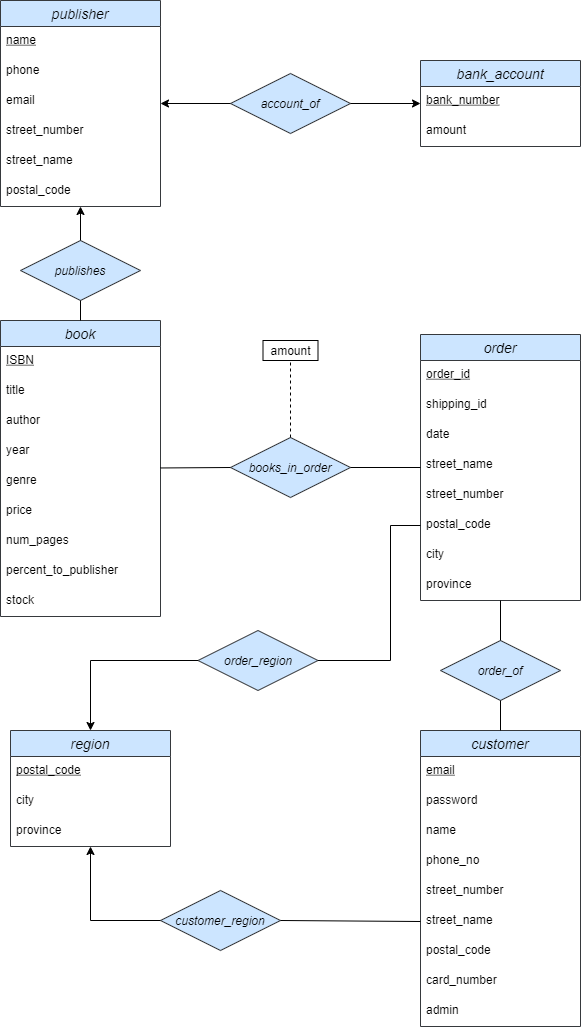
\includegraphics[scale=0.4]{../Diagrams/ER-diagram-bookstore-comp3005-finalproject-after-normalization.drawio.png}\\

\section{Database Schema Diagram}

The following is the Schema Diagram created to model schemas gained from our ER diagram and after normalization.\\

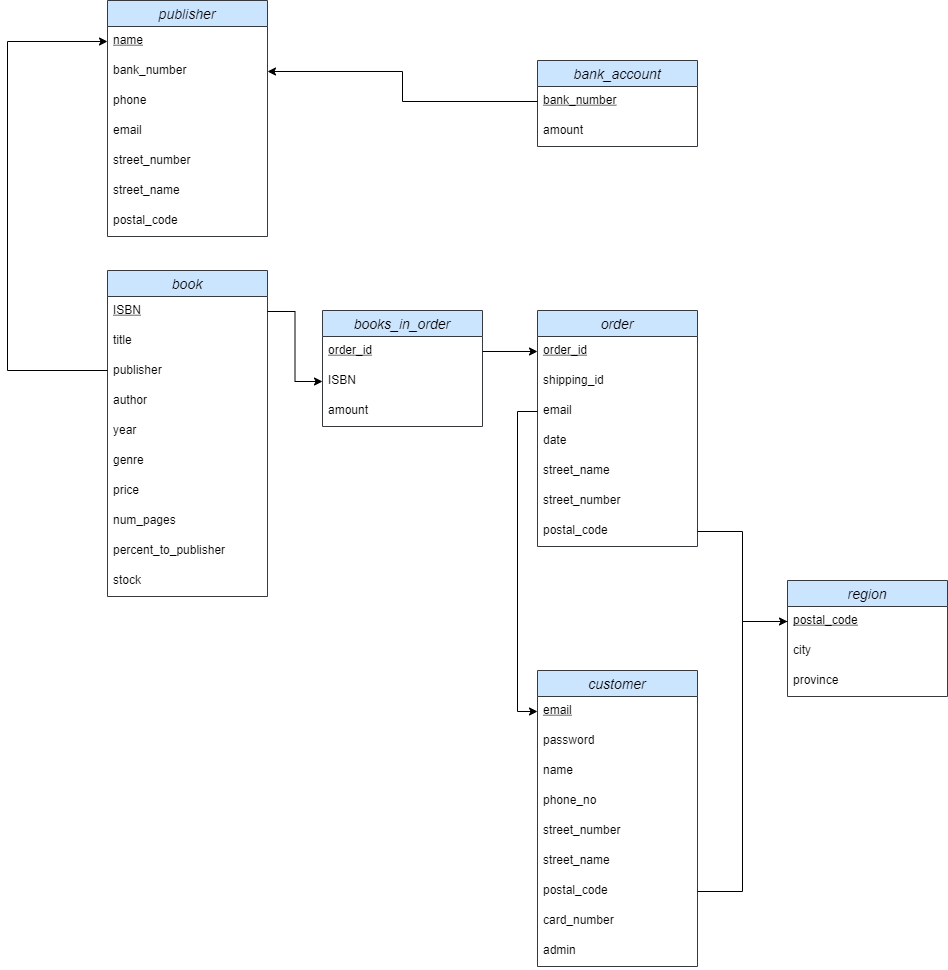
\includegraphics[scale=0.5]{../Diagrams/Schema-diagram-comp3005-finalproject-after-normalization.drawio.png}\\

\section{Implementation}
\underline{\textbf{Implementation Design}}
In this section we will briefly mention how we implemented certain features of our bookstore and what SQL elements were used to achieve this.\\

For our orders, the primary key that is used for the order relation is the order\_id. The order\_id is created immediately upon the creation of a new order into the table. We achieved this by making use of the "serial" datatype in our table.\\

Regarding the book stock, whenever the book's stock level goes below a certain threshold (ex. in our case we set it to below 10 books), an order needs to be placed to restock the books inventory. To achieve this, we implemented an SQL trigger on the book relation that activates whenever on stock of a book goes below 10. The trigger performs this check whenever a book entry is updated.\\

For publisher reports, we supported three different types of reports. Sales vs Expenditures (which is just amount in bank\_account vs debt\_amount), Sales vs Authors and Sales vs Genres. For the last two reports, we implemented SQL functions that would return us a table with Authors/Genres and Sales for those given authors or genres. The function takes in a varchar argument that is the name of the publisher to retrieve the results for. Whenever a user requests to see the reports page for a specific publisher, we call those functions and pass in the specific publisher as the name. We also thought of using a view to do this, however we chose the route of SQL functions.\\

\underline{\textbf{Implementation Tour}}\\
The following are a few screen shots showing what the user and owner would see when browsing the website.\\

\noindent\emph{Customer Perspective}\\
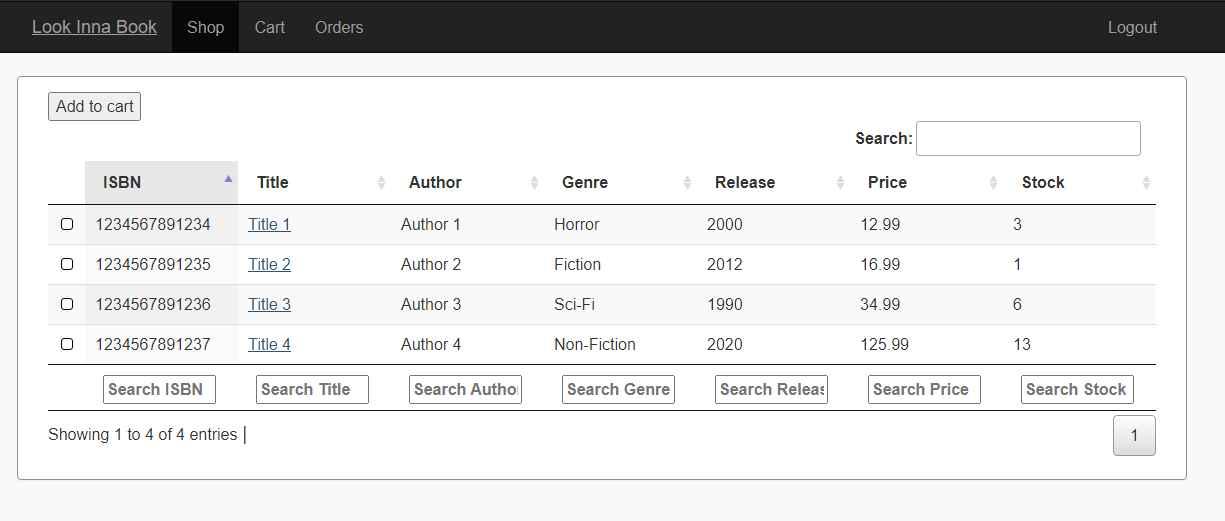
\includegraphics[scale=0.5]{../Images/user_book_page.png}\\

\noindent\emph{Owner Perspective}\\
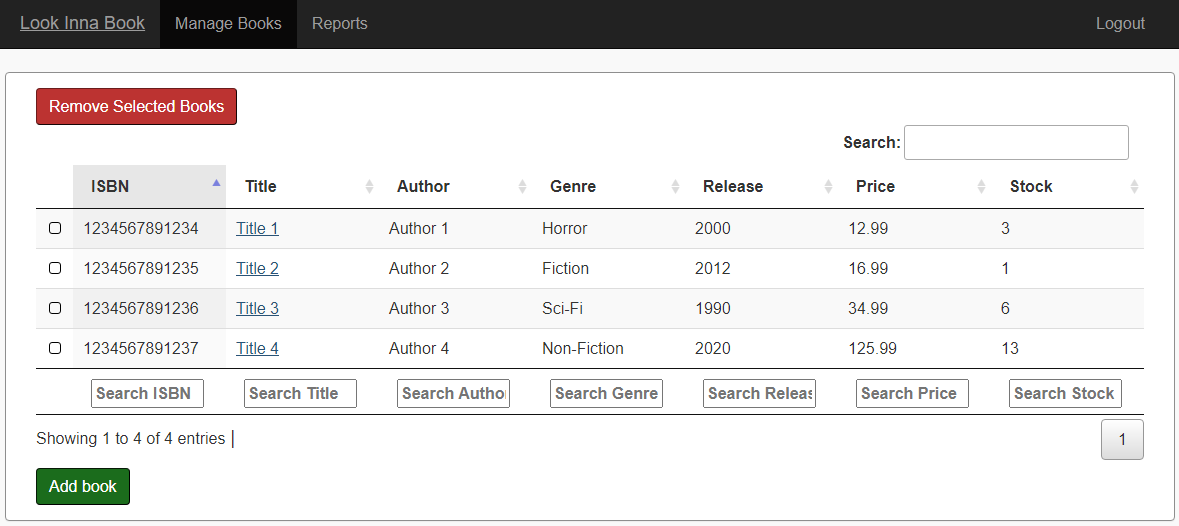
\includegraphics[scale=0.5]{../Images/owner_book_page.png}\\

\noindent\underline{Video Tour}\\
The following is a video tour of the bookstore website. It walks through all the main features of the bookstore and demonstrates specific functionality mentioned in the problem statement.\\

\noindent\href{https://www.youtube.com/}{View video here...}\\
EDIT THIS!!!\\

\section{Github Repository}
\noindent All project files and source code can be found at the following \href{https://github.com/COMP3005A-Project/bookstore}{Github repository}...

\section{Appendix I}
Below are a list of three available time slots for December 18th 2021 (one day after the "implied" due date of Dec 17th 2021), for possible project demonstrations...
\begin{itemize}
	\item 11:00AM - 11:20AM
	\item 12:00PM - 12:20PM
	\item 01:00PM - 01:20PM
\end{itemize}

\end{document}